Web-Browser haben sich seit der Veröffentlichung von Mosaic, einem der ersten populären Browser, im Jahr 1993 stark weiterentwickelt \cite{EvolutionOfTheWebBrowser}. Das Abrufen und Anzeigen von statischen HTML-Dokumenten wurde mithilfe von JavaScript um interaktive und später um dynamische Inhalte erweitert. Mittels JavaScript können Entwickler heutzutage komplexe browser-unabhängige Webanwendungen realisieren \cite{SinglePageApplication}. Diese Entwicklung hat den Browser als populäre Laufzeitumgebung für Anwendungen über alle Betriebssysteme und Plattformen hinweg etabliert \cite{TheWebAsAnApplicationPlatform}.

%\subsection{Browserprodukte}
%\label{sec:browserprodukte}

%\begin{wrapfigure}[19]{r}{0.45\textwidth}
%\centering
%\tikzsetnextfilename{cross-browser_metastudie.png}
%\begin{tikzpicture}
%	\begin{axis}[
%		ybar,
%        ymin=0,
%        ymax=300,
%        ytick distance={50},
%		area style,
%		legend style={at={(0.5,-0.10)},anchor=north},
%		nodes near coords,
%		symbolic x coords = {2015, 2016, 2017, 2018, 2019, 2020},
%	]
%		\addplot+[blue,fill opacity=0.2,text opacity=1,ybar,no marks]
%			plot coordinates {
%			(2015,272)
%			(2016,228)
%			(2017,208)
%			(2018,204)
%			(2019,172)
%			(2020,167)
%			};
%		\legend{\strut Suchtreffer bei Google Scholar}
%	\end{axis}
%\end{tikzpicture}
%\caption{Studien zur Browserkompatibilität, eigene Darstellung (vgl. \ref{sec:studien-zur-browser-kompatibilitaet})}
%\label{fig:studien-zur-browser-kompatibilitaet}
%\end{wrapfigure}

\vspace{\baselineskip}

\begin{wrapfigure}[18]{r}{0.45\textwidth}
\centering
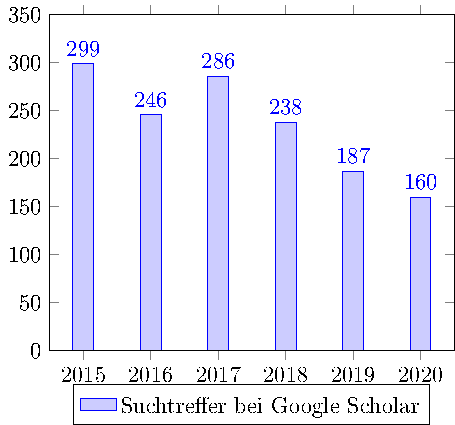
\includegraphics[width=\linewidth]{img/02_theorie/cross-browser_metastudie.png.pdf}
\caption{Studien zur Browserkompatibilität, eigene Darstellung (vgl. \autoref{sec:studien-zur-browser-kompatibilitaet})}
\label{fig:studien-zur-browser-kompatibilitaet}
\end{wrapfigure}

Die Vielfalt an Browsern bereitet Webentwicklern immer wieder Herausforderungen bei dem Ziel ein einwandfrei funktionierendes Produkt, unabhängig der Browserpräferenz des Nutzers, bereitzustellen. Die Häufigkeit solcher Probleme, auch Cross-Browser-Incompatibilities (XBI) \cite{XBIs} genannt, hat jedoch abgenommen. Dies ist unter anderem durch den Trend von offenen Web-Standards, wie die des W3C \cite{W3CStandards}, erklärbar.

\nomenclature[Fachbegriff]{XBI}{Cross-Browser-Incompatibilities}

Generell lässt sich feststellen, dass auch in der Literatur die Veröffentlichungen in Bezug auf (In-)Kompatibilität von Browsern abnehmen, wie in \autoref{fig:studien-zur-browser-kompatibilitaet} zu betrachten ist. Dies spricht dafür, dass das Problem von XBIs weniger präsent ist als zuvor. Somit wird die besondere Hürde, die XBIs darstellen, in dieser Arbeit als nicht relevant angesehen.

\pagebreak

Im Jahr 2020 gab es eine wesentliche Entwicklung, die die Kompatibilität zwischen Browsern erhöhen und Unterschiede zukünftig spürbar reduzieren wird. Microsoft ist beim Folgeprodukt zum Internet Explorer, dem Microsoft Edge, von einer proprietären Browser-Engine zu Chromium gewechselt \cite{MicrosoftEdgeChromium} und verwendet somit denselben Kern wie die Browser Chrome und Opera. Zudem stellte Microsoft zum 30.11.2020 den Support für den Internet Explorer 11 ein \cite{MicrosoftInternetExplorerDeprecation}.

Eine Übersicht der aktuellen Browser mit Marktnteil und den verwendeten Engines für Layout und JavaScript, kann in \autoref{tab:uebersicht-der-aktuellen-browser} betrachtet werden. Hierbei wird deutlich, dass der überwiegende Anteil (>95\%) der Desktop-Browser auf den Engines Blink, WebKit und Gecko bzw. für JavaScript auf V8, JavaScriptCore und SpiderMonkey basieren.

\begin{table}[H]
\centering
\begin{tabular}{|l|l|l|l|}
  \hline
  Browser & Anteil        & Layout-Engine  & JavaScript-Engine \\
  \hline
  Chrome  & 66,47\%       & Blink          & V8                \\
  \hline
  Safari  & 10,27\%       & WebKit         & JavaScriptCore    \\
  \hline
  Firefox & 8,17\%        & Gecko          & SpiderMonkey      \\
  \hline
  Edge    & 8,01\%        & Blink          & V8                \\
  \hline
  Opera   & 2,68\%        & Blink          & V8                \\
  \hline
  Internet Explorer & 1,89\% & Trident     & Chakra            \\
  \hline
\end{tabular}
\caption{Übersicht aktueller Browser \cite{StatCounterBrowserMarketshare} \cite{CompatibilityAndDefaults}}
	\label{tab:uebersicht-der-aktuellen-browser}
\end{table}